\section*{Maneouver study}
\addcontentsline{toc}{section}{Maneouver study}
Let us assume symmetric flight (no lateral aerodynamic force $Q=0$ nor lateral thrust force as $\nu=0$), the thrust generated by the engines is parallel to the \textit{x} wind axis (thus $\epsilon=0$),  and that the maneuver takes place flawlessly, this is in the vertical plane too; $\xi=\dot{\xi}=0$.\\
As the maneuver is a rather short, we will also assume that the fuel consumed i negligible and no mass fraction is lost; $\dot{m}=0$.
 
The three force configurations during the maneuver correspond to the free body diagrams at stages 1, 2 and 3 (see Figure \ref{fig:immelmann-overview}). \vspace{0.5cm}

%\begin{minipage}{\textwidth}
	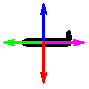
\includegraphics[width=0.3\linewidth]{figures/free-body-1.pdf} \hfill
%	\captionof{subfigure}{Angles evolution over time}
	\label{fig:free-body-1}
		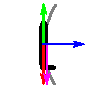
\includegraphics[width=0.3\linewidth]{figures/free-body-2.pdf}\hfill
%	\captionof{subfigure}{Angles evolution over time}
	\label{fig:free-body-2}
		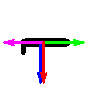
\includegraphics[width=0.3\linewidth]{figures/free-body-3.pdf}
%	\captionof{subfigure}{Angles evolution over time}
	\label{fig:free-body-3}
	\vspace{0.5cm}
%\end{minipage}

Note that at all times the lift behaves as the centripetal force, thus indicating that both the velocity and radius limitations to perform the Immelmann turn are inherent to the wing design and its maximum and minimum lift generation.\\
As a result, the radius can be writen as a function of the angle of attack. By operating with the third equation of system number \ref{eq:semicircle}, which is in wind system of reference, very convenient as is also polar system:
\begin{align*}
	L=&m\left(\frac{V^2}{R}+g\cos(\gamma)\right)\\
	\frac{1}{2}\rho S V^2 C_L(\alpha)=&m\left(\frac{V^2}{R}+g\cos(\gamma)\right)\\
	R=&\frac{2mV^2}{2W\cos(\gamma)+\rho S V^2 C_L(\alpha)}
\end{align*}
As the plane must describe a semicircle, the radius must be constant.